\documentclass[tikz,border=2pt]{standalone}
\usepackage{amsmath}
\usetikzlibrary{arrows.meta, decorations.pathreplacing}
\begin{document}
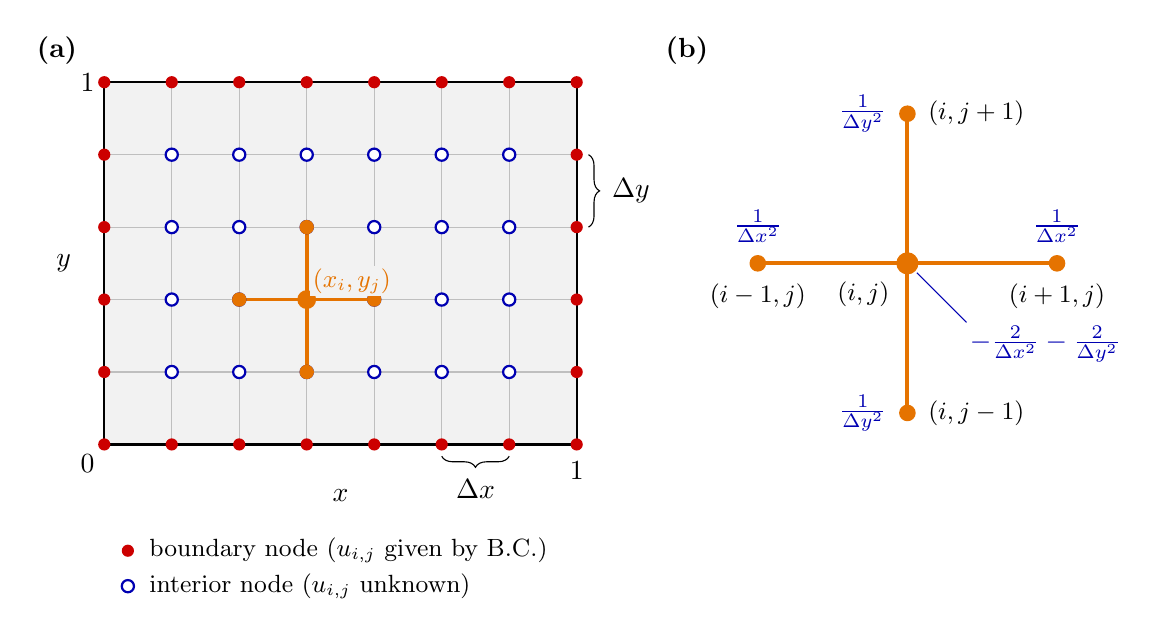
\begin{tikzpicture}[>=Stealth]
% ---------------- (a) grid on the unit square ----------------
\begin{scope}
    \def\Nx{7} \def\Ny{5}          % number of intervals in x and y
    \def\W{6} \def\Hh{4.6}          % drawn width and height of the square
    \pgfmathsetmacro{\dx}{\W/\Nx}
    \pgfmathsetmacro{\dy}{\Hh/\Ny}
    % domain and grid lines
    \fill[gray!10] (0,0) rectangle (\W,\Hh);
    \foreach \i in {1,...,6} \draw[gray!50] (\i*\dx,0) -- (\i*\dx,\Hh);
    \foreach \j in {1,...,4} \draw[gray!50] (0,\j*\dy) -- (\W,\j*\dy);
    \draw[thick] (0,0) rectangle (\W,\Hh);
    % stencil at (i,j) = (3,2)
    \def\ci{3} \def\cj{2}
    \draw[line width=1.4pt, orange!90!black]
        ({(\ci-1)*\dx},{\cj*\dy}) -- ({(\ci+1)*\dx},{\cj*\dy})
        ({\ci*\dx},{(\cj-1)*\dy}) -- ({\ci*\dx},{(\cj+1)*\dy});
    % boundary nodes (Dirichlet data)
    \foreach \i in {0,...,7} {
        \fill[red!80!black] (\i*\dx,0) circle (2.2pt);
        \fill[red!80!black] (\i*\dx,\Hh) circle (2.2pt);
    }
    \foreach \j in {1,...,4} {
        \fill[red!80!black] (0,\j*\dy) circle (2.2pt);
        \fill[red!80!black] (\W,\j*\dy) circle (2.2pt);
    }
    % interior nodes (unknowns)
    \foreach \i in {1,...,6} \foreach \j in {1,...,4}
        \filldraw[fill=white, draw=blue!70!black, thick] (\i*\dx,\j*\dy) circle (2.2pt);
    % highlight stencil nodes
    \foreach \a/\b in {-1/0, 1/0, 0/-1, 0/1}
        \fill[orange!90!black] ({(\ci+\a)*\dx},{(\cj+\b)*\dy}) circle (2.6pt);
    \fill[orange!90!black] ({\ci*\dx},{\cj*\dy}) circle (3.4pt);
    \node[orange!90!black, above right=1pt, font=\small, fill=gray!10, inner sep=1pt]
        at ({\ci*\dx},{\cj*\dy}) {$(x_i, y_j)$};
    % spacing annotations
    \draw[decorate, decoration={brace, amplitude=4pt, mirror}]
        ({5*\dx},-0.15) -- ({6*\dx},-0.15) node[midway, below=5pt] {$\Delta x$};
    \draw[decorate, decoration={brace, amplitude=4pt}]
        ({\W+0.15},{4*\dy}) -- ({\W+0.15},{3*\dy}) node[midway, right=5pt] {$\Delta y$};
    % axis labels
    \node[below left] at (0,0) {$0$};
    \node[below] at (\W,-0.1) {$1$};
    \node[left] at (0,\Hh) {$1$};
    \node[below] at ({\W/2},-0.45) {$x$};
    \node[left] at (-0.3,{\Hh/2}) {$y$};
    % legend
    \begin{scope}[shift={(0.3,-1.35)}, font=\small]
        \fill[red!80!black] (0,0) circle (2.2pt);
        \node[right] at (0.15,0) {boundary node ($u_{i,j}$ given by B.C.)};
        \filldraw[fill=white, draw=blue!70!black, thick] (0,-0.45) circle (2.2pt);
        \node[right] at (0.15,-0.45) {interior node ($u_{i,j}$ unknown)};
    \end{scope}
    \node[font=\bfseries] at (-0.6,\Hh+0.4) {(a)};
\end{scope}

% ---------------- (b) the 5-point stencil ----------------
\begin{scope}[xshift=10.2cm, yshift=2.3cm]
    \def\s{1.9}
    \draw[line width=1.4pt, orange!90!black] (-\s,0) -- (\s,0) (0,-\s) -- (0,\s);
    \foreach \a/\b in {-1/0, 1/0, 0/-1, 0/1}
        \fill[orange!90!black] (\a*\s,\b*\s) circle (3pt);
    \fill[orange!90!black] (0,0) circle (4pt);
    % node indices
    \node[below=4pt, font=\small] at (-\s,0) {$(i-1, j)$};
    \node[below=4pt, font=\small] at (\s,0) {$(i+1, j)$};
    \node[right=4pt, font=\small] at (0,\s) {$(i, j+1)$};
    \node[right=4pt, font=\small] at (0,-\s) {$(i, j-1)$};
    \node[below left=3pt, font=\small] at (0,0) {$(i,j)$};
    % weights
    \node[above=4pt, blue!70!black] at (-\s,0) {$\frac{1}{\Delta x^2}$};
    \node[above=4pt, blue!70!black] at (\s,0) {$\frac{1}{\Delta x^2}$};
    \node[left=4pt, blue!70!black] at (0,\s) {$\frac{1}{\Delta y^2}$};
    \node[left=4pt, blue!70!black] at (0,-\s) {$\frac{1}{\Delta y^2}$};
    \draw[blue!70!black, thin] (0.12,-0.12) -- (0.75,-0.75);
    \node[anchor=north west, blue!70!black, inner sep=1pt] at (0.75,-0.75)
        {$-\frac{2}{\Delta x^2} - \frac{2}{\Delta y^2}$};
    \node[font=\bfseries] at (-\s-0.9,\s+0.8) {(b)};
\end{scope}
\end{tikzpicture}
\end{document}
